% =============================================================================
% Huawei ICT Competition — Innovation Track (Regional)
% Standalone Overleaf project (NOT the BAU thesis in research/main.tex)
% =============================================================================
\documentclass[11pt,a4paper]{article}

\usepackage[T1]{fontenc}
\usepackage[utf8]{inputenc}
\usepackage{lmodern}
\usepackage[margin=2.5cm]{geometry}
\usepackage{microtype}
\usepackage{silence}
\WarningFilter{latex}{Command \showhyphens has changed}
\usepackage{graphicx}
\usepackage{booktabs}
\usepackage{tabularx}
\usepackage{array}
\usepackage{enumitem}
\usepackage{xurl}
\usepackage[breaklinks]{hyperref}
\hypersetup{colorlinks=true, linkcolor=blue, urlcolor=blue, citecolor=blue}
\usepackage{listings}
\usepackage{caption}
\usepackage{subcaption}
\usepackage[numbers,sort&compress]{natbib}
\usepackage{tikz}
\usetikzlibrary{positioning, arrows.meta}

\lstset{
  basicstyle=\ttfamily\small,
  breaklines=true,
  frame=single,
  tabsize=2,
  showstringspaces=false
}

% ------------- Team / institution (edit names) -------------
\newcommand{\TeamName}{SYNSheild}
\newcommand{\Institution}{Beirut Arab University (BAU), Lebanon}
\newcommand{\SubmissionDate}{11 April 2026}
\newcommand{\MemberOneName}{Wafik Ibrahim}
\newcommand{\MemberOneRole}{PCAP pipeline, dataset construction, labeling scripts}
\newcommand{\MemberTwoName}{Mohammed Farhat}
\newcommand{\MemberTwoRole}{MindSpore training, evaluation, checkpoints}
\newcommand{\MemberThreeName}{Abed Al Rida Nehme}
\newcommand{\MemberThreeRole}{Reporting, reproducibility, deployment integration}
\newcommand{\AdvisorName}{Ali Nassar (instructor)}
% -------------------------------------------------------------

% Show a framed placeholder if optional image files are not uploaded yet
\newcommand{\optionalfig}[3][0.92\linewidth]{%
  \IfFileExists{#2}{%
    \includegraphics[width=#1]{#2}%
  }{%
    \fbox{\parbox[c][3.0cm][c]{#1}{\centering\small\sffamily [#3]\\[0.35em]\footnotesize\path{#2}}}%
  }%
}

\title{%
  Huawei MindSpore \& ResNeXt-50: SYN-Flood DDoS Detection\\
  from PCAP Packet Images\\[0.5em]
  \large Huawei ICT Competition --- Innovation Track (Regional)}
\author{\TeamName\\\Institution}
\date{\SubmissionDate}

\bibliographystyle{unsrtnat}

\begin{document}
\maketitle

\begin{abstract}
\noindent\textbf{Team \TeamName.} Distributed Denial of Service (DDoS) attacks, especially TCP SYN floods, threaten service availability. This project delivers an end-to-end pipeline that converts raw network captures (PCAP) into fixed-size grayscale images and classifies them with a ResNeXt-50 (32$\times$4d) model trained in Huawei MindSpore~\cite{mindspore} using mindcv~\cite{mindcv}. The work targets the ICT Innovation track~\cite{ictcompetition}: a concrete problem, a working software pipeline, and measurable offline performance on the public CICDDoS2019 dataset~\cite{cicddos2019}.

\textbf{Primary benchmark:} a model trained on \textbf{0.3\,s time-window} images, evaluated on held-out validation and test splits from the same distribution, plus a blind random sample from the test split. On the test split (1845 samples), the system reaches \textbf{98.10\%} accuracy and \textbf{0.9375} macro F1; a blind test of 270 images (maximum balanced sample, seed 42) yields \textbf{98.9\%} accuracy and \textbf{0.9889} macro F1.

A legacy \textbf{per-packet} configuration achieves very high scores on a large blind test (3000 images); \textbf{cross-domain} experiments show that mixing image constructions without retraining does not transfer. Operational deployments must use the \textbf{same} preprocessing as training.
\end{abstract}

\tableofcontents
\clearpage

\section{Competition alignment (Innovation track)}

\begin{table}[h]
  \centering
  \small
  \begin{tabular}{@{}p{0.28\linewidth}p{0.62\linewidth}@{}}
    \toprule
    Expectation & How this project addresses it \\
    \midrule
    Real problem & SYN flood DDoS and availability risk \\
    Creative solution & Packet bytes $\rightarrow$ 2D image $\rightarrow$ ResNeXt; class-balanced training; 0.3\,s windows \\
    Implementation & PCAP scripts, MindSpore + mindcv, training and eval tooling \\
    Evidence & Metrics, confusion matrices, blind tests, optional calibration \\
    Feasibility & Cross-domain results and deployment caveats documented \\
    \bottomrule
  \end{tabular}
\end{table}

\section{Problem statement and objectives}

\paragraph{Problem.}
Attackers send large volumes of TCP SYN segments to exhaust server resources. Operators need automated aids beyond brittle static rules alone.

\paragraph{Objectives.}
\begin{enumerate}[leftmargin=*]
  \item Binary classification: DDoS (SYN flood) vs.\ normal from PCAP data.
  \item Train a ResNeXt-50 classifier with \textbf{Huawei MindSpore}.
  \item Evaluate on CICDDoS2019 with train/validation/test splits and blind inference.
  \item Document reproducibility for regional review.
\end{enumerate}

\paragraph{Non-goals.}
Full SOC integration, exhaustive evasion studies, and multi-attack-type detection are out of scope but noted as future work.

\section{Project identity and regional context}

\paragraph{Team brand.}
\textbf{\TeamName} (pronounced like ``SYN shield'') is the competing team's project name: it highlights protection against abusive \textbf{SYN} traffic while remaining memorable for judges and audiences.

\paragraph{Institution and region.}
The project is developed at \textbf{Beirut Arab University (BAU)} in \textbf{Lebanon}. Reliable network services matter for education, finance, and public infrastructure in the region; tools that help operators spot SYN-flood patterns earlier support broader \textbf{digital resilience} goals. Participation in the \textbf{Huawei ICT Competition} Innovation track~\cite{ictcompetition} frames this work as student-led engineering with a clear path from dataset to reproducible evaluation.

\section{Related work}

Public DDoS corpora and taxonomies (e.g.\ Sharafaldin et al.~\cite{sharafaldin2018developing}) motivated realistic evaluation; CICDDoS2019~\cite{cicddos2019} continues that lineage. Deep learning for intrusion and traffic analysis is surveyed broadly~\cite{vinayakumar2019deep}; CNN-style models on transformed traffic representations are common. Lotfollahi et al.~\cite{lotfollahi2020deep} illustrate how raw byte-level views can feed deep networks (in their case encrypted-traffic classification). Closer to this project, Bazzi et al.~\cite{bazzi2020resnet} encode SYN-flood-related packets as grayscale images and classify with ResNet on CICDDoS2019. \textbf{Our work} swaps ResNet-50 for \textbf{ResNeXt-50}, implements the stack in \textbf{MindSpore + mindcv}, adds an automated PCAP-to-image pipeline with class imbalance handling, and studies \textbf{time-window} images (0.3\,s) as the primary deployment-facing representation.

\section{Innovation and differentiation}

\begin{enumerate}[leftmargin=*]
  \item \textbf{Architecture.} Prior related work used ResNet-50~\cite{bazzi2020resnet}; we use \textbf{ResNeXt-50 (32$\times$4d)} (grouped convolutions / cardinality).
  \item \textbf{Huawei stack.} MindSpore + mindcv supports Ascend / Huawei Cloud deployment narratives where relevant.
  \item \textbf{End-to-end automation.} Zipped CICDDoS2019 $\rightarrow$ PCAP heuristics $\rightarrow$ images $\rightarrow$ training/evaluation scripts.
  \item \textbf{Security metrics.} Weighted cross-entropy, optional \textbf{focal-loss} training runs (checkpoint directory \path{per_second_0p3_focal_v2}), and macro-F1 checkpoint selection.
  \item \textbf{Temporal variant.} 0.3\,s window images are the \textbf{primary} model; a separate \textbf{1\,s} window experiment exists in the repository scripts but is not the headline result here. Legacy \textbf{per-packet} results are retained for comparison. Cross-domain evaluation shows train/deploy \textbf{representation alignment} is mandatory.
\end{enumerate}

\section{System overview}

\begin{enumerate}[leftmargin=*]
  \item \textbf{Ingest:} PCAP files (e.g.\ CICDDoS2019).
  \item \textbf{Label (heuristic):} PCAPs exceeding a SYN-packet threshold $\rightarrow$ DDoS for dataset construction (Appendix~\ref{app:pipeline}).
  \item \textbf{Convert:} Raw bytes arranged as 2D grayscale, resized to $224{\times}224$~\cite{bazzi2020resnet}.
  \item \textbf{Train:} ResNeXt-50, ImageNet-style preprocessing, Adam / AdamWeightDecay, weighted (and optionally focal) loss.
  \item \textbf{Evaluate:} Val/test metrics, blind draws, optional ROC/PR/calibration (see Figure~\ref{fig:rocpr} when the PDF asset is included).
\end{enumerate}

\begin{figure}[ht]
  \centering
  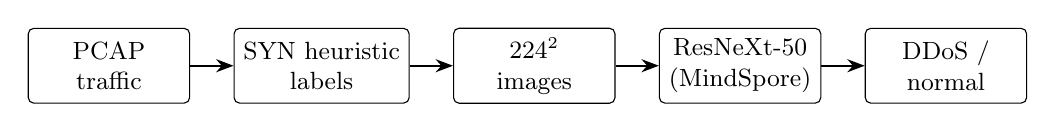
\begin{tikzpicture}[
    node distance=0.9cm and 0.55cm,
    box/.style={
      rectangle, draw=black, rounded corners=2pt,
      minimum height=0.95cm, minimum width=2.05cm,
      align=center, font=\small
    },
    arr/.style={-{Stealth[length=2.2mm]}, thick}
  ]
    \node[box] (pcap) {PCAP\\traffic};
    \node[box, right=of pcap] (lab) {SYN heuristic\\labels};
    \node[box, right=of lab] (img) {$224^2$\\images};
    \node[box, right=of img] (rn) {ResNeXt-50\\(MindSpore)};
    \node[box, right=of rn] (out) {DDoS /\\normal};
    \draw[arr] (pcap) -- (lab);
    \draw[arr] (lab) -- (img);
    \draw[arr] (img) -- (rn);
    \draw[arr] (rn) -- (out);
  \end{tikzpicture}
  \caption{End-to-end pipeline: capture $\rightarrow$ dataset labels $\rightarrow$ packet/window images $\rightarrow$ classifier $\rightarrow$ decision.}
  \label{fig:pipeline}
\end{figure}

\paragraph{Primary artifacts for judging.}
Checkpoint \path{model/per_second_0p3_focal_v2/resnext50_32x4d_best.ckpt}; data root \path{dataset/images_per_second_window_0p3/}.

\section{Illustrative figures}

Figure~\ref{fig:samples} shows two \textbf{224$\times$224} grayscale inputs from our \textbf{0.3\,s} time-window pipeline on CICDDoS2019: \textbf{normal} traffic (left) and \textbf{SYN-flood DDoS} (right). Source exports: \texttt{syn0} vs.\ high SYN-count window (\texttt{syn8204}). Figure~\ref{fig:rocpr} shows \textbf{ROC} and \textbf{precision--recall} curves on the held-out \textbf{test} split, produced by \texttt{scripts/eval\_roc\_pr\_calibration.py} (via \texttt{bash scripts/run\_all\_paper\_figures.sh}); PDFs are mirrored under \texttt{figures/} as \texttt{roc\_test.pdf} and \texttt{pr\_test.pdf}.

\begin{figure}[ht]
  \centering
  \begin{subfigure}[t]{0.48\textwidth}
    \centering
    \optionalfig[0.95\linewidth]{figures/sample_normal.png}{Add normal sample}
    \caption{Normal (benign) --- 0.3\,s window}
  \end{subfigure}\hfill
  \begin{subfigure}[t]{0.48\textwidth}
    \centering
    \optionalfig[0.95\linewidth]{figures/sample_ddos.png}{Add DDoS sample}
    \caption{SYN-flood DDoS --- 0.3\,s window}
  \end{subfigure}
  \caption{Example time-window images from CICDDoS2019 (normal vs.\ DDoS).}
  \label{fig:samples}
\end{figure}

\begin{figure}[ht]
  \centering
  \begin{subfigure}[t]{0.48\textwidth}
    \centering
    \optionalfig[0.95\linewidth]{figures/roc_test.pdf}{Add ROC PDF}
    \caption{ROC (test split)}
  \end{subfigure}\hfill
  \begin{subfigure}[t]{0.48\textwidth}
    \centering
    \optionalfig[0.95\linewidth]{figures/pr_test.pdf}{Add PR PDF}
    \caption{Precision--recall (test split)}
  \end{subfigure}
  \caption{ROC and PR curves for the primary 0.3\,s model on the test split.}
  \label{fig:rocpr}
\end{figure}

\section{Dataset and methodology (summary)}

\paragraph{Dataset.}
CICDDoS2019~\cite{cicddos2019}: public, realistic benign and attack traffic including SYN floods.

\paragraph{Splits.}
Folders \texttt{train/}, \texttt{val/}, \texttt{test/} with subfolders \texttt{ddos/} and \texttt{normal/}. Class indices follow \textbf{alphabetical} order (\texttt{ddos}=0, \texttt{normal}=1).

\paragraph{Model.}
ResNeXt-50 32$\times$4d; input $224{\times}224$ RGB (grayscale replicated to three channels); two-class softmax.

\paragraph{Training highlights (primary 0.3\,s run).}
Optimizer Adam / AdamWeightDecay; learning rate $10^{-3}$, weight decay $10^{-4}$; batch size 16; 8 epochs; weighted cross-entropy; the saved \textbf{best} weights use the run tagged \path{focal_v2} in the output directory (focal loss used during that training trajectory). Checkpoint selection uses \textbf{macro F1} on validation. Full tables: Appendix~\ref{app:train}.

\section{Results}

\subsection[Primary model (0.3 s time-window)]{Primary model --- 0.3\,s time-window images}

\noindent\textbf{Checkpoint:} \path{model/per_second_0p3_focal_v2/resnext50_32x4d_best.ckpt}.\\
\textbf{Evaluation recorded:} 2026-04-03 (GPU; Appendix~\ref{app:repro}).

\begin{table}[h]
  \centering
  \caption{Primary model --- validation and test}
  \begin{tabular}{@{}lrrr@{}}
    \toprule
    Split & Samples & Accuracy & Macro F1 \\
    \midrule
    Validation & 1842 & 98.21\% & 0.9399 \\
    Test       & 1845 & 98.10\% & 0.9375 \\
    \bottomrule
  \end{tabular}
\end{table}

\begin{table}[h]
  \centering
  \caption{Test confusion matrix (rows = true, columns = predicted)}
  \begin{tabular}{@{}lrr@{}}
    \toprule
     & pred.\ ddos & pred.\ normal \\
    \midrule
    true ddos   & 135 & 0 \\
    true normal & 35  & 1675 \\
    \bottomrule
  \end{tabular}
\end{table}

\begin{table}[h]
  \centering
  \caption{Per-class precision and recall on the \textbf{test} split (derived from the confusion matrix)}
  \label{tab:perclass}
  \begin{tabular}{@{}lrrr@{}}
    \toprule
    Class & Precision & Recall & F1 \\
    \midrule
    DDoS  & 0.794 & 1.000 & 0.885 \\
    Normal & 1.000 & 0.979 & 0.990 \\
    \bottomrule
  \end{tabular}
\end{table}

\noindent\textbf{Blind test} (\path{blind_test_random.py}, test split, seed 42, 270 images): 267/270 correct (98.9\%); macro F1 0.9889.

\subsection{Comparison to simple and prior baselines}

Table~\ref{tab:baseline} contrasts the primary model with (i) a \textbf{majority baseline} that always predicts the most frequent test class (\texttt{normal}) on the same 1845 test samples, and (ii) the \textbf{Bazzi et al.} ResNet-50 packet-image line~\cite{bazzi2020resnet} (reported strong CICDDoS2019 accuracy in their setting; exact numbers depend on their split and preprocessing, so we quote qualitatively). The majority baseline illustrates why accuracy alone is misleading under imbalance.

\begin{table}[h]
  \centering
  \caption{Sanity check vs.\ trivial baseline on the \textbf{same} 0.3\,s test split ($n=1845$).}
  \label{tab:baseline}
  \small
  \begin{tabular}{@{}p{0.36\linewidth}rrr@{}}
    \toprule
    Method & Accuracy & Macro F1 \\
    \midrule
    Always predict \texttt{normal} & 92.7\% & 0.481 \\
    Bazzi et al.\ ResNet-50~\cite{bazzi2020resnet} &
      \multicolumn{2}{>{\raggedright\arraybackslash}p{0.52\linewidth}}{%
        Reported strong CICDDoS2019 accuracy in their ResNet image setup; split and preprocessing differ from ours, so we do not paste a single competing scalar here.} \\
    \textbf{Ours ResNeXt-50 (primary)} & \textbf{98.10\%} & \textbf{0.9375} \\
    \bottomrule
  \end{tabular}
\end{table}

\subsection{Legacy model --- per-packet images (reference)}

Per-packet images under \texttt{dataset/images/}: test macro F1 $\approx$ 95.56\%. Large blind test of 3000 images: 99.9\% accuracy, macro F1 0.9993. These apply only to the per-packet checkpoint; not interchangeable with the 0.3\,s model without matching preprocessing (Appendix~\ref{app:legacy}).

\subsection{Calibration (optional)}

Scripts can produce ROC/PR and calibration diagnostics (e.g.\ test ECE $\approx$ 0.074, heuristic threshold $\approx$ 0.87 for max F1 in one logged run). See Appendix~\ref{app:figs}.

\section{Operational inference (offline)}

Batch evaluation for the primary checkpoint was run on a \textbf{NVIDIA GeForce RTX 3070} with MindSpore 2.6.0 (Appendix~\ref{app:repro}). Throughput depends on dataloader and disk I/O; in practice, evaluating the full test split is \textbf{interactive} (seconds to a few minutes), not hours. For competition demos, report wall-clock time from your machine with \path{scripts/eval_test_detailed.py} if you need a concrete number. Ascend or cloud deployment would use the same graph after export---out of scope here beyond noting MindSpore compatibility.

\section{Limitations, risks, and ethics}

\begin{enumerate}[leftmargin=*]
  \item \textbf{Dataset scope.} Metrics reflect CICDDoS2019 and labeling heuristics; production traffic may differ.
  \item \textbf{Representation alignment.} Cross-domain evaluation shows poor transfer when test images differ from training construction.
  \item \textbf{Heuristic labels.} SYN counts are a proxy for dataset building, not operator ground truth.
  \item \textbf{Privacy.} PCAPs may contain sensitive data; handle per institutional policy.
  \item \textbf{Adversarial robustness} not evaluated here.
\end{enumerate}

\section{Demo, deployment, and reproducibility}
\label{sec:deploy}

\paragraph{Minimal offline story.}
PCAPs $\rightarrow$ images $\rightarrow$ ResNeXt in MindSpore $\rightarrow$ confusion matrices and F1 on held-out data plus blind sampling.

\paragraph{Live service caveat.}
If you operate \path{run_pipeline.py} or a systemd service under \path{depployemnt/}, confirm whether live windows use \textbf{per-packet} images or the same \textbf{0.3\,s aggregation} as training. Internal evaluation notes document a mismatch risk: \textbf{reported headline metrics} apply to the \textbf{offline 0.3\,s image} pipeline. Align windowing with training before claiming live parity.

\begin{lstlisting}[language=bash,caption={Reproduce primary metrics}]
cd /path/to/huawei
bash scripts/run_all_eval_0p3.sh
\end{lstlisting}

\noindent Extended commands and versions: Appendix~\ref{app:eval} and \path{reports/REPRODUCIBILITY.md} in the repository.

\section{Future work}

Strictly align live capture with the 0.3\,s training representation or retrain on the live representation; extend to multi-class DDoS families or encrypted traffic; formal latency/throughput benchmarks on GPU and Ascend; deeper Huawei Cloud packaging if later stages require it.

\section{Team and contributions}

\begin{itemize}[leftmargin=*]
  \item \textbf{\MemberOneName} --- \MemberOneRole
  \item \textbf{\MemberTwoName} --- \MemberTwoRole
  \item \textbf{\MemberThreeName} --- \MemberThreeRole
  \item \textbf{Advisor:} \AdvisorName
\end{itemize}


\bibliography{references}

\clearpage
\appendix
% Appendix for ICT Innovation report (included from main.tex)
% Compile: pdflatex + bibtex + pdflatex x2 (Overleaf does this automatically)

\section{Document map}
\label{app:map}

\begin{table}[h]
  \centering
  \small
  \begin{tabular}{@{}ll@{}}
    \toprule
    File & Purpose \\
    \midrule
    \texttt{SYSTEM\_DESCRIPTION.txt} & Canonical internal system description (repo root) \\
    \texttt{reports/eval\_results\_per\_second\_0p3.md} & Primary 0.3\,s evaluation log \\
    \texttt{reports/cross\_domain\_eval\_2026-04-03.md} & Cross-domain study \\
    \texttt{reports/REPRODUCIBILITY.md} & Environment snapshot \\
    \texttt{reports/pip\_freeze\_2026-04-03.txt} & Frozen dependencies (if present) \\
    \texttt{reports/paper\_figures\_2026-04-03.log} & Calibration / figure run log \\
    \bottomrule
  \end{tabular}
\end{table}

\section{Reproducibility snapshot (2026-04-03)}
\label{app:repro}

\begin{table}[h]
  \centering
  \begin{tabular}{@{}ll@{}}
    \toprule
    Item & Value \\
    \midrule
    Git commit & \texttt{96b82d4cf152053175950a346bdd204b6e109ebf} \\
    Python & 3.10.12 \\
    MindSpore & 2.6.0 \\
    mindcv & 0.3.0 \\
    GPU (eval machine) & NVIDIA GeForce RTX 3070 \\
    NVIDIA driver & 535.288.01 \\
    CUDA toolkit (typical) & \texttt{/usr/local/cuda-11.6} \\
    \bottomrule
  \end{tabular}
\end{table}

\noindent
Full \texttt{pip freeze}: regenerate on your machine or use the dated file under \texttt{reports/}.
Install MindSpore using the official matrix at \url{https://www.mindspore.cn/install/en}, then \texttt{pip install -r requirements.txt} for \texttt{mindcv}, NumPy, Pillow.

\section{Data processing pipeline (detailed)}
\label{app:pipeline}

\begin{enumerate}[leftmargin=*]
  \item \textbf{Source archives:} CICDDoS2019 zips in batches (\texttt{scripts/process\_zips\_in\_batches.sh}).
  \item \textbf{PCAP labeling:} \texttt{scripts/classify\_pcap\_syn.py} --- PCAPs with $>100$ TCP SYN packets $\rightarrow$ DDoS, else normal.
  \item \textbf{Packet selection:} DDoS PCAPs use SYN-only conversion (\texttt{--syn-only}); normal uses all packets.
  \item \textbf{Image conversion:} \texttt{scripts/pcap\_to\_images.py} --- raw bytes to $224{\times}224$ grayscale; driver \texttt{scripts/convert\_pcaps\_to\_images.sh}.
  \item \textbf{Layout:} \texttt{train/}, \texttt{val/}, \texttt{test/} with \texttt{ddos/} and \texttt{normal/}.
  \item \textbf{Time-window variant:} \texttt{dataset/images\_per\_second\_window\_0p3/} (0.3\,s) --- primary training distribution.
\end{enumerate}

\section{Training configuration}
\label{app:train}

\noindent\textbf{Entry point:} \texttt{notebook/train\_resnext.py}.\\
\textbf{Model:} ResNeXt-50 32$\times$4d via mindcv.

\noindent\textbf{Preprocessing:} train: RandomResizedCrop(224), RandomHorizontalFlip; eval/test: resize 256 then center crop 224; ImageNet normalization.

\noindent\textbf{Documented run:} MindSpore (Graph mode); Adam / AdamWeightDecay; lr $10^{-3}$, weight decay $10^{-4}$; batch 16; 8 epochs; weighted cross-entropy; best checkpoint by macro F1 on validation.

\begin{table}[h]
  \centering
  \begin{tabular}{@{}ll@{}}
    \toprule
    Role & Path \\
    \midrule
    Primary (0.3\,s) & \path{model/per_second_0p3_focal_v2/resnext50_32x4d_best.ckpt} \\
    Legacy per-packet & \path{model/resnext50_32x4d_best.ckpt} \\
    \bottomrule
  \end{tabular}
\end{table}

\noindent
Some eval scripts enforce the primary checkpoint; non-primary override may require environment variable \path{HUAWEI_EVAL_ALLOW_NON_PRIMARY_CKPT=1}.

\section[Primary evaluation, extended tables (0.3 s)]{Primary evaluation --- extended tables (0.3\,s)}
\label{app:eval}

Source: \texttt{scripts/eval\_test\_detailed.py}.

\subsection*{Validation (1842 samples)}
Overall accuracy 0.982085; macro F1 0.939942; weighted F1 0.982986; balanced accuracy 0.990345.

\begin{table}[h]
  \centering
  \begin{tabular}{@{}lrr@{}}
    \toprule
     & pred.\ ddos & pred.\ normal \\
    \midrule
    true ddos & 133 & 0 \\
    true normal & 33 & 1676 \\
    \bottomrule
  \end{tabular}
\end{table}

\noindent Per-class F1: ddos 0.889632; normal 0.990251.

\subsection*{Test (1845 samples)}
Overall accuracy 0.981030; macro F1 0.937453; weighted F1 0.982020; balanced accuracy 0.989766.

\begin{table}[h]
  \centering
  \begin{tabular}{@{}lrr@{}}
    \toprule
     & pred.\ ddos & pred.\ normal \\
    \midrule
    true ddos & 135 & 0 \\
    true normal & 35 & 1675 \\
    \bottomrule
  \end{tabular}
\end{table}

\noindent Per-class F1: ddos 0.885246; normal 0.989660.

\subsection*{Blind test (270 images, seed 42)}
Accuracy $267/270$ (98.9\%); macro F1 0.9889. Confusion: ddos 135/0; normal 3/132.

\begin{lstlisting}[language=bash,caption={Reproduce primary metrics (GPU example)}]
cd /path/to/huawei
bash scripts/run_all_eval_0p3.sh
\end{lstlisting}

\begin{lstlisting}[language=bash,caption={Individual eval calls (adjust venv)}]
.venv/bin/python scripts/eval_test_detailed.py \
  --ckpt model/per_second_0p3_focal_v2/resnext50_32x4d_best.ckpt \
  --data-root dataset/images_per_second_window_0p3 --split val --device-target GPU
.venv/bin/python scripts/eval_test_detailed.py \
  --ckpt model/per_second_0p3_focal_v2/resnext50_32x4d_best.ckpt \
  --data-root dataset/images_per_second_window_0p3 --split test --device-target GPU
.venv/bin/python scripts/blind_test_random.py \
  --data-root dataset/images_per_second_window_0p3 \
  --ckpt model/per_second_0p3_focal_v2/resnext50_32x4d_best.ckpt \
  --split test --total 270 --seed 42 --device-target GPU
\end{lstlisting}

\section{Legacy per-packet evaluation (reference)}
\label{app:legacy}

Test macro F1 $\approx$ 95.56\%. Small blind test $5{+}5$ images, seed 42: 10/10. Large blind test 3000 images (1500/class):

\begin{table}[h]
  \centering
  \begin{tabular}{@{}lrr@{}}
    \toprule
     & pred.\ ddos & pred.\ normal \\
    \midrule
    true ddos & 1498 & 2 \\
    true normal & 0 & 1500 \\
    \bottomrule
  \end{tabular}
\end{table}

\noindent Accuracy 2998/3000 (99.9\%); macro F1 0.9993.

\begin{lstlisting}[language=bash]
python scripts/blind_test_random.py --data-root ./dataset/images --split test --total 3000
\end{lstlisting}

\section{Cross-domain evaluation}
\label{app:cross}

Recorded 2026-04-03 with \texttt{scripts/eval\_cross\_domain.py --device-target GPU}.

\subsection*{G.1 --- 0.3\,s checkpoint on per-packet test}
19300 samples; accuracy 0.987565 (majority normal); macro F1 0.496872; balanced accuracy 0.500000. Argmax never predicted DDoS (misleading headline accuracy).

\subsection*{G.2 --- Per-packet checkpoint on 0.3\,s test}
1845 samples; accuracy 0.898645; macro F1 0.473309; DDoS recall 0 under argmax.

\begin{lstlisting}[language=bash,caption={Cross-domain reproduction}]
cd /path/to/huawei
export CUDA_HOME=/usr/local/cuda-11.6
export PATH="$CUDA_HOME/bin:$PATH"
.venv/bin/python scripts/eval_cross_domain.py \
  --ckpt model/per_second_0p3_focal_v2/resnext50_32x4d_best.ckpt \
  --train-order-root dataset/images_per_second_window_0p3 \
  --eval-root dataset/images --split test --device-target GPU
.venv/bin/python scripts/eval_cross_domain.py \
  --ckpt model/resnext50_32x4d_best.ckpt \
  --train-order-root dataset/images \
  --eval-root dataset/images_per_second_window_0p3 --split test --device-target GPU
\end{lstlisting}

\section{Figures and calibration}
\label{app:figs}

Run \texttt{bash} \path{scripts/run_all_paper_figures.sh}; figures are written under \path{research/figures/}.
See \path{reports/paper_figures_2026-04-03.log} for test ECE $\approx$ 0.074 and heuristic threshold $\approx$ 0.87 for max F1 (reconfirm if re-run).

\section{Script index}
\label{app:scripts}

\small
\begin{tabular}{@{}>{\raggedright\arraybackslash}p{0.42\linewidth}>{\raggedright\arraybackslash}p{0.52\linewidth}@{}}
  \toprule
  Path & Role \\
  \midrule
  \path{notebook/train_resnext.py} & Training / eval entry \\
  \path{scripts/classify_pcap_syn.py} & PCAP labeling \\
  \path{scripts/pcap_to_images.py} & Bytes $\rightarrow$ image \\
  \path{scripts/convert_pcaps_to_images.sh} & Batch conversion \\
  \path{scripts/process_zips_in_batches.sh} & Zip batching \\
  \path{scripts/blind_test_random.py} & Blind sampling eval \\
  \path{scripts/eval_test_detailed.py} & Detailed metrics \\
  \path{scripts/eval_cross_domain.py} & Cross-domain \\
  \path{scripts/eval_roc_pr_calibration.py} & ROC/PR/calibration \\
  \path{scripts/eval_primary_ckpt.py} & Checkpoint policy \\
  \path{scripts/run_all_eval_0p3.sh} & One-shot primary eval \\
  \path{scripts/run_all_paper_figures.sh} & Figures \\
  \path{run_pipeline.py} & Live/offline pipeline \\
  \path{depployemnt/} & Deployment helpers \\
  \bottomrule
\end{tabular}
\normalsize

\section{Repository layout (abbreviated)}
\label{app:tree}

\begin{verbatim}
huawei/
  notebook/train_resnext.py
  scripts/
  model/per_second_0p3_focal_v2/resnext50_32x4d_best.ckpt
  model/resnext50_32x4d_best.ckpt
  dataset/images/
  dataset/images_per_second_window_0p3/
  reports/
  research/
  requirements.txt
  SYSTEM_DESCRIPTION.txt
\end{verbatim}

\section{Glossary}
\label{app:gloss}

\begin{itemize}[leftmargin=*]
  \item \textbf{PCAP:} Packet capture file.
  \item \textbf{SYN flood:} TCP handshake exhaustion attack pattern.
  \item \textbf{Macro F1:} Unweighted mean of per-class F1 scores.
  \item \textbf{Time-window image:} Packets in a short window (0.3\,s) aggregated into one image.
  \item \textbf{Per-packet image:} One image per packet (legacy setup).
  \item \textbf{Blind test:} Random sample; model sees images only.
\end{itemize}

\section{Deployment note}
\label{app:deploy}

See Section~\ref{sec:deploy} in the main report for the distinction between \textbf{offline 0.3\,s metrics} and a possible \textbf{live} \path{run_pipeline.py} / service path.

If a remote demo exists, provide judge access via a non-public handout if credentials are required. Live \texttt{pred: ddos} lines on unlabeled traffic are not confirmed attacks---domain shift and thresholding apply.


\end{document}
